\section{Algorithms}
\label{sec:algorithms}

% \red{\textit{The first part contains the detailed discussion and the
%     mathematical description of the used algorithms. The second part contains
%     the recipe algorithm, i.e. a high-level description of the recipe
%     flow-chart and how it changes for different parameter settings.}}

\subsection{General Algorithms}
\label{sec:algorithms-general}

\subsection{Optimal Extraction}
\label{sec:extract}
\begin{figure}[ht]
    \begin{center}
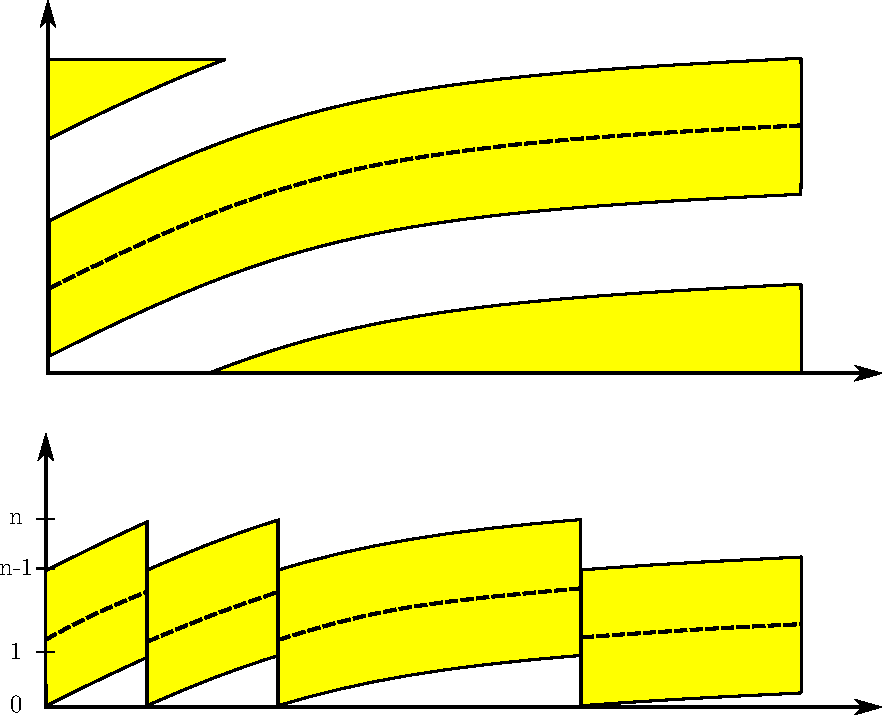
\includegraphics[width=0.45\linewidth]{rectification.pdf}
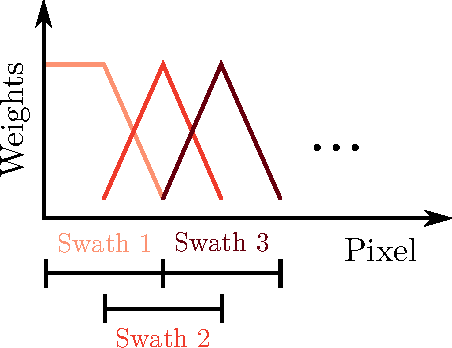
\includegraphics[width=0.45\linewidth]{swath_weights.pdf}
\end{center}
\caption{\it Left: Illustration of swath rectification. Right: The weights 
    for combining the spectra from overlapping swaths.}
\label{fig:swaths}
\end{figure}

\begin{figure}[ht]
    \begin{center}
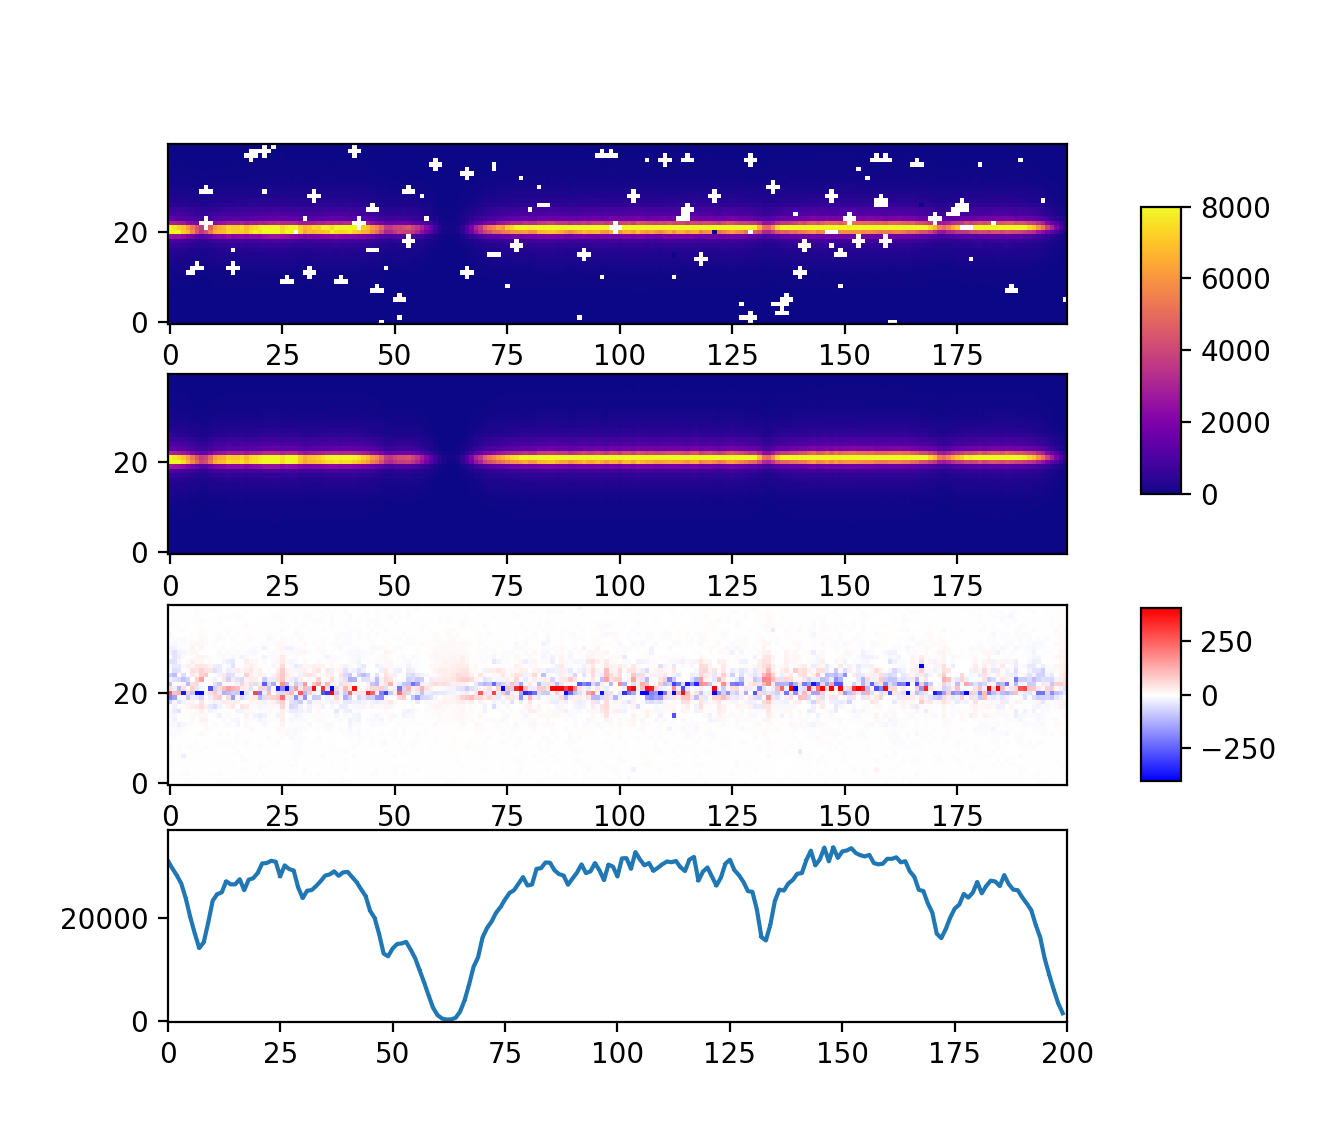
\includegraphics[width=0.85\linewidth]{extr_model.png}
\end{center}
\caption{An example of the optimal extraction. \emph{Top:} The flat-fielded,
combined, and pair-wise subtracted frame, with the BPM applied and zoomed-in to
part of a single spectral order. \emph{Panel 2:} The model of the same region,
reconstructed from the extracted spectrum and slit-function. \emph{Panel 3:} The
difference between the two above, showing the residuals. \emph{Bottom:} The
extracted spectrum itself, on the same x-axis as the panels above.}
\label{fig:extrmodel}
\end{figure}

The optimal extraction along the tilted and curved slit is a centerpiece of the
\instrument\ DRS and several recipes make use of it. Full details and
mathematical description can be found in \cite{2021A&A...646A..32P}. Here, we
simply summarize the most important practical implications from a user
perspective.

To extract a spectral order from a calibrated 2D frame into a 1D spectrum, using
a \emph{trace} from the TW table, the following steps are carried out:
\begin{itemize}
    \item Calculate the extraction height from the edge-polynomials, if not
    explicitly given via \texttt{-{}-extract\_height}.
    \item Cut out a rectangular region around the mid-line, called a
    \emph{swath} from the frame, using the height and the value of
    \texttt{-{}-extract\_swath\_width}.
    \item Rectify the swath by shifting columns by integer values such that the
    mid-line only retains values between $0\ldots 1$, like illustrated in
    \figref{fig:swaths} (left).
    \item Iteratively approximate the swath surface by two vectors: the spectrum
    along the mid-line and the slit-function along the slit projection, taking
    its changing tilt into account. The slit function is oversampled by a factor
    \verb!--extract_oversample!.
    \item Step by a half swath-width to the next one, and repeat. This way
    swaths overlap fully and the order effectively gets extracted twice.
    \item Once all swaths are extracted, the spectra from each are merged into
    one, with linearly in-/decreasing weights, as in \figref{fig:swaths}
    (right).
    \item The spectrum and slit-functions are saved, and used to reconstruct a
    2D model of the frame, saved separately.
    \item The errors are estimated from the residual between data and model.
\end{itemize}

A major advantage of this extraction algorithm is that it makes no assumption
about the slit-function, except that it does not change within a swath. This
allows, for example, to combine jittered nodding frames into one, and extract it
together.

In addition, the model by design cannot approximate features that are not
present in all pixels that contribute to a certain bin in the spectrum or the
slit-function. This makes spectra robust towards e.g.~cosmic rays.

Fig.~\ref{fig:varyovers} shows the effect of the \emph{slit-function
oversampling}, that can be changed via  the parameter \linebreak
\verb!--extract_oversample!. As mentioned before, this factor linearly affects
the computation time. The amount of oversampling necessary depends on how
quickly the mid-line of a spectral order changes with respect to detector rows,
and how sharply the slit-function changes. The default value of $5$ is enough in
many situations, but clearly leaves artifacts in the example shown, which was
chosen to be close to worst-case, and requires an oversampling $>12$ for optimal
results.

\putgraph{.8\linewidth}{varyoversample.pdf}{varyovers}{Example spectrum,
 extracted with varying oversampling, and vertically offset for plotting.
 In this case, oversampling of $12$ is needed to no longer see "spiky" artifacts.}

There are a few more parameters that influence the extraction:
\begin{itemize}
    \item \verb!--extract_swath_width! sets the width of the swath, in pixels,
    i.e.~how large a piece of a spectral order should be processed at a time.
    Meaningful values range from $~50$ (high S/N necessary) to the full detector
    width. The default is $800$ and works in most cases, because the
    slit-illumination rarely varies on that scale.
    \item \verb!--extract_height! sets the height in pixels of the extracted
    region, symmetrical around the mid-line of the trace. By default, this is
    not set and the upper and lower edge polynomials of the trace are used to
    set the height. Setting this parameter therefore overrides the role of the
    edge polynomials in the extraction.
    \item \verb!--extract_smooth_slit! is a regularization parameter for the
    slit-illumination vector, as it is approximated during the extraction. The
    value is roughly the size of the smoothing kernel in pixels, and should not
    be set below $1.0$ to avoid ringing. Default is $2.0$.
    \item \verb!--extract_smooth_spec! is analogous to the previous, but along
    the spectrum instead. It defaults to $0.0$ to not degrade resolution, but
    can be increased as needed.
\end{itemize}

For the utility recipe \verb!cr2res_util_extract! these parameters are named
without the prefix \verb!extract_!.

\subsection{Other extraction methods}
\label{sec:otherextr}

\verb!cr2res_util_extract! has another feature up its sleeve: the parameter
\verb!--method! which allows using different algorithms to extract spectra from
the 2D frame. It can take the following values.
\begin{itemize}
    \item \verb!SUM!, a simple vertical sum of the spectral order. Because of
    the non-vertical slit, spectral features will be broadened.
    \item \verb!MEDIAN!, same as previous, but calculating the median instead of
    the sum. The value is multiplied by the extraction height, so that the
    normalization is the same as the other methods.
    \item \verb!TILTSUM! is like \verb!SUM!, but first shifts the detector rows
    according to the slit tilt. Only integer shifts, so there is still smoothing
    from sub-pixel tilt.
    \item \verb!OPT_VERT! should not be used! It runs the optimal extraction
    along a vertical slit, but is not optimized for speed and therefore slower
    than
    \item \verb!OPT_CURV!, the default optimal extraction, as described above.
\end{itemize}

For all other recipes, \verb!OPT_CURV! is the only choice.

\subsection{Errors and Signal-to-Noise}
\label{sec:errors}

Raw frames contain pixel values in ADU. All data products are in ADU also,
i.e.~no conversion to electrons is made, and no normalization to $1s$-exposure by
dividing by \verb!DIT!. There are however several steps along the way to the
final spectra that affect the absolute values of pixels and spectral bins, which
is why it makes sense to summarize them here.

Some things to keep in mind about ADU values
\begin{itemize}
    \item For data with \verb!NDIT >1!, each sub-exposure gets averaged in the
    detector software.
    \item In a nodding sequence the pair-wise subtracted frames are also
    averaged.
    \item The normalization of the output-spectra is like that of a sum of pixel
    values, collapsed along the slit, i.e. summed-up ADU.
\end{itemize}


Errors, both in maps and spectra are absolute. Calibrations are applied to raw
frames in the following order, at each step propagating the error into the
output
\begin{itemize}
    \item Bad pixel map\footnote{BPMs have no errors, therefore no
    error-propagation at this step.}
    \item Detector non-linearity.
    \item Shot-noise gets added to each pixel's error, based on $\sqrt{\verb!ADU!}$
    divided by $\sqrt{\verb!NDIT!}$ and $\sqrt{\verb!GAIN!}$.
    \item Dark-subtraction. The master darks are DETLIN-corrected, because they
    are not "dark" but contain thermal emission.
    \item Optional subtraction of all detector rows with a row, that is derived
    by taking the vertical median over the 40 bottom rows which receive no
    light.
    \item Division by the normalized flat-field.
    \item Optional correction for cosmic rays (usually not necessary).
\end{itemize}


The errors of each pixel are used in the optimal extraction, and once that is
done, a \emph{model} gets reconstructed from the spectrum and the slit-function.
The residual between data and model gets quadratically added to the pixel
uncertainties, which in turn get divided by the slit function to become the
error of the spectral bin.

This means that the spectrum can be directly divided by the error-spectrum to
obtain the signal-to-noise ratio (S/N). No further conversions are necessary.

However, in order to compare this S/N with the theoretical expectation from
Poissonian statistics, users will have to scale the ADU-values of the spectrum
by the gain and the number of averaged frames (NDIT or combined frames), before
taking the square-root (Eq.~\ref{eq:snr}). In general, the measured S/N after extraction is
somewhat lower than the theoretical value.

\begin{equation}
    \label{eq:snr}
    S/N = \sqrt{(ADU_A+ADU_B)*NDIT*NEXP*NABCYCLES*GAIN}\quad ,
\end{equation}
where $ADU_{A,B}$ are the spectra from nodding positions A and B, respectively.
For other types of observations replace accordingly. Polarimetric observations
always take four exposures at different SPU-angles; the demodulated intensity
spectrum (Stokes I) therefore needs an additional factor 4 in the equation.

\subsection{Recipes Algorithms} 
\label{sec:algorithms-recipes}


\subsubsection{Order Tracing}
\label{sec:ordertrace}

As written above, by a \emph{trace}, we mean a polynomial, in pixel-coordinates
of a single detector, that follows the mid-line of a spectral order. And two
more polynomials for the upper and lower edges of the slit projection, as shown
in Fig.~\ref{fig:flat_trace}.

The way this is derived is by first determining which pixels in a FLAT frame
contain signal, and which don't. To that end the image is smoothed first
horizontally, then vertically, and then compared to the unsmoothed frame via
thresholding.

After that it is determined which spectral order the pixels belong to. For this
purpose, the mean Y-coordinate for each order is present in the raw file
headers.

Lastly, the X and Y-coordinates for pixels within the same order are fitted with
a polynomial, which gives the mid-line of the trace. In addition, edge-detection
gives the upper and lower edges of the spectral order.

\subsubsection{Measuring the slit-tilt}
\label{sec:tilt}

The recipe \verb!cr2res_util_slit_curv! takes as input a TW, for the order
traces, and an FPET frame. The algorithm finds the etalon peaks, which give good
coverage in each spectral order. It then fits the shape of each peak with a
polynomial P(y), because in principle a curved slit could cross the same
x-coordinate more than once.

The coefficients of these polynomials are then fitted with a P(x) for each
degree. This ensures a smooth change of the slit tilt with wavelength, removes
outliers, and allows to store the information in the TW in an analogous way to
the polynomials for trace and wavelength solution. The TW-columns are named
\verb!SlitPolyA!, \verb!SlitPolyB! and \verb!SlitPolyC!.


\subsubsection{Wavelength calibration}

\putgraph{\linewidth}{wavecal_resids_H1567.png}{waveresids}{An example of residual values after wavelength calibration with the FPET.}

There are several ways to calibrate the wavelength scale, and each corresponds
to one of the values that the parameter \texttt{-{}-wl\_method} of
\texttt{cr2res\_util\_wave} can take.

With \texttt{-{}-wl\_method=XCORR} the provided catalog of lines is converted
into a synthetic spectrum that is cross-correlated with the extracted lamp
spectrum. Each detector-order is calibrated separately.

degree=0, which means a shift of the zero-point only, keeping the polynomial coefficients for the higher degrees fixed.
TODO
keep=true with XCORR.
fallback

The line catalogs for Uranium lines come from \cite{2018A&A...618A.118S} and
\cite{2011ApJS..195...24R}. They are used for YJ and HK-bands, respectively.
Note that all wavelengths are vacuum, not air.



The recipe \texttt{cr2res\_cal\_wave} executes several steps after one another that can be replicated with individual calls of util-recipes:

\begin{itemize}
    \item apply master calibrations to raw (UNE and FPET) frames, \verb!cr2res_util_calib!
    \item extract spectra from the calibrated frames, \verb!cr2res_util_extract!
    \item calibrate UNE with XCORR and degree=0, which means a shift of the zero-p
    
\end{itemize}

TODO

combines two methods into one recipe, one
for the UNE lamp frames, and the one for the FPET. The result from the former
gets passed on to the latter, if both lamp inputs are present. If not, then only
the appropriate method is applied. 


for the L and M-bands, the TW
molecfit

\subsubsection{Detector non-linearity}
\label{sec:detlin}

\putgraph{.8\linewidth}{detlin_1133_1564.png}{detlincorr}{Before and after
 non-linearity correction for a randomly picked pixel in each detector. Red
 circles: Raw ADU/s vs.~ADU. Green dots with errorbars: ADU/s as read from FLATs
 to which the previously derived calibration has been applied, using
 \texttt{cr2res\_util\_calib}. The closer to horizontal the points fall, the
 better the correction, because the actual illumination is kept constant. The
 standard-deviation from 1 is given in the title. Diamonds and shaded region: As
 a cross-check, the plotting-script separately reads and applies the correction
 to the raw values; should align with green dots and errors.}


Users are provided (via the data archive) with the calibration data-product
(\verb!PRO.CATG=CAL_DETLIN_COEFFS!) that is needed to apply the correction for
the non-linear response of detector pixels. This file contains for each pixel
the coefficients of a polynomial which, when evaluated at a certain ADU-level,
yields the correction factor by which to multiply the raw ADU, so that the value
becomes that which a linear response would have given.

The \verb!cr2res_obs_*! recipes take
this file as optional input and apply the correction, so do some of the
calibration recipes, most notably \verb!cr2res_cal_flat!. Since there is a
degeneracy between the pixel response characterized by the normalized flat-field
and the detlin-coefficients, users are advised to provide the detlin to either
\emph{both} the flat-field and science reductions, or to \emph{neither} of them.


In order to derive this correction, a long series of exposures with the
flat-field lamp are taken, with increasing DITs, starting from very short until
well into saturation. This is repeated for several spectrograph settings in
order to cover the gaps between the spectral orders. A series of DARKs with
matching DIT is also obtained and subtracted from the FLATS, because the
non-zero detector background pattern at short DITs would otherwise influence the
determination of the linear response.

The reduction of the data set is done by \verb!cr2res_cal_detlin!
\begin{shell}[fontsize=\footnotesize]
    %prompt cat detlin.sof
    CRIRE.2021-10-18T09:50:30.827.fits DETLIN_LAMP
    CRIRE.2021-10-18T09:50:32.845.fits DETLIN_LAMP
    ...
    CRIRE.2021-10-18T09:59:12:345.fits DETLIN_DARK
    ...

    %prompt esorex cr2res_cal_detlin detlin.sof
\end{shell}

For each pixel, the recipe carries out the following steps on the sequence of images:
\begin{itemize}
    \item Convert ADU to ADU/s by dividing by DIT. Plotting ADU/s versus ADU
    gives a horizontal line in the linear regime (illuminating flux is kept
    constant), and deviates downward for larger ADU (Fig.~\ref{fig:detlincorr}).
    \item Assume linear response up to 4000 ADU and take median of all
    measurements below this threshold to find the \emph{true ADU/s}.
    \item Divide the non-linear ADU/s by the true value to get the correction
    factors, depending on ADU-level.
    \item Fit a parabola to the correction factors' dependence on ADU.
    \item Save the coefficients into data product.
\end{itemize}

This procedure is repeated for the other spectrograph settings and in the end
the coefficients are merged, with weights according to their errors.


\putgraph{.8\linewidth}{detlin_corrfacs.png}{detlincorrfac}{The size of the
non-linearity correction, depending on raw ADU-level.}


\putgraph{.8\linewidth}{detlin_errmaps.png}{detlinerrmap}{Error maps for three
ADU levels. These are the propagated errors of the correction factor for each
pixel, at that ADU. Clearly visible are the spectral orders and gaps, with the
largest errors for the pixels that are only illuminated by one of the three
spectrograph settings.}


\putgraph{.8\linewidth}{detlin_accur.png}{detlinaccur}{How well does a known
constant illumination get recovered by applying the correction? This is what the
deviation from the horizontal line at 1.0 in this figure shows. A value of 1.005
on the y-axis corresponds to 0.5\% inaccuracy. Points are average deviations of
random pixels for a certain ADU-bin; errorbars here are the standard-deviation
of values in the same bin, not the propagated errors.}

The additional figures \ref{fig:detlinerrmap}, \ref{fig:detlincorrfac} and \ref{fig:detlinaccur} show some statistics of the outcome.
For example, one way to read these figures is that at 30,000 ADU, a correction
of around 10\% needs to be applied, and this correction is accurate to around
0.5\%. 
